% -----------------------------------------------
% Template for SMC 2019
% adaed from the template for SMC 2018
% -----------------------------------------------

\documentclass{article}
\usepackage{smc2019}
\usepackage{times}
\usepackage{ifpdf}
\usepackage[english]{babel}
\usepackage{cite}
\usepackage{physics}
\usepackage{tikz}
\usepackage{tikz-qtree}
\usetikzlibrary{trees}% cfr added this as the code fails to compile otherwise

%%%%%%%%%%%%%%%%%%%%%%%% Some useful packages %%%%%%%%%%%%%%%%%%%%%%%%%%%%%%%
%%%%%%%%%%%%%%%%%%%%%%%% See related documentation %%%%%%%%%%%%%%%%%%%%%%%%%%
\usepackage{amsmath} % popular packages from Am. Math. Soc. Please use the 
\usepackage{amssymb} % related math environments (split, subequation, cases,
\usepackage{amsfonts}% multline, etc.)
\usepackage{bm}      % Bold Math package, defines the command \bf{}
\usepackage[]{algorithm2e}
%\usepackage{paralist}% extended list environments
%%subfig.sty is the modern replacement for subfigure.sty. However, subfig.sty 
%%requires and automatically loads caption.sty which overrides class handling 
%%of captions. To prevent this problem, preload caption.sty with caption=false 
%\usepackage[caption=false]{caption}
%\usepackage[font=footnotesize]{subfig}


%user defined variables
\def\papertitle{Real-time Control of Advanced Physical Models using the Sensel Morph}
\def\firstauthor{Silvin Willemsen}
\def\secondauthor{Nikolaj Andersson }
\def\thirdauthor{Stefania Serafin}
\def\fourthauthor{Stefan Bilbao}

% adds the automatic
% Saves a lot of output space in PDF... after conversion with the distiller
% Delete if you cannot get PS fonts working on your system.

% pdf-tex settings: detect automatically if run by latex or pdflatex
\newif\ifpdf
\ifx\pdfoutput\relax
\else
   \ifcase\pdfoutput
      \pdffalse
   \else
      \pdftrue
\fi

\ifpdf % compiling with pdflatex
  \usepackage[pdftex,
    pdftitle={\papertitle},
    pdfauthor={\firstauthor, \secondauthor, \thirdauthor, \fourthauthor},
    bookmarksnumbered, % use section numbers with bookmarks
    pdfstartview=XYZ % start with zoom=100% instead of full screen; 
                     % especially useful if working with a big screen :-)
   ]{hyperref}
  %\pdfcompresslevel=9

%   \usepackage[pdftex]{graphicx}
  % declare the path(s) where your graphic files are and their extensions so 
  %you won't have to specify these with every instance of \includegraphics
  \graphicspath{{./figures/}}
  \DeclareGraphicsExtensions{.pdf,.jpeg,.png,.eps}

  \usepackage[figure,table]{hypcap}

\else % compiling with latex
  \usepackage[dvips,
    bookmarksnumbered, % use section numbers with bookmarks
    pdfstartview=XYZ % start with zoom=100% instead of full screen
  ]{hyperref}  % hyperrefs are active in the pdf file after conversion

  \usepackage[dvips]{epsfig,graphicx}
  % declare the path(s) where your graphic files are and their extensions so 
  %you won't have to specify these with every instance of \includegraphics
  \graphicspath{{./LATEX/}}
  \DeclareGraphicsExtensions{.eps}

  \usepackage[figure,table]{hypcap}
\fi

%setup the hyperref package - make the links black without a surrounding frame
\hypersetup{
    colorlinks,%
    citecolor=black,%
    filecolor=black,%
    linkcolor=black,%
    urlcolor=black
}
\SetAlCapSkip{1em}
% inkscape -D -z --file=JUCE.svg --export-pdf=JUCESVG.pdf --export-latex

% Title.
% ------
\title{\papertitle}

% Authors
% Please note that submissions are NOT anonymous, therefore 
% authors' names have to be VISIBLE in your manuscript. 
%
% Single address
% To use with only one author or several with the same address
% ---------------
% \twoauthors
%   {Silvin Willemsen, Nikolaj Andersson and Stefania Serafin} { \\ Multisensory Experience Lab, CREATE, Aalborg University Copenhagen \\ %
%     {\tt \href{mailto:sil@create.aau.dk}{\{sil, nsa, sts\}@create.aau.dk}}}

% Two addresses
% --------------
\oneauthor
  {\firstauthor, \secondauthor and \thirdauthor} {Multisensory Experience Lab,\\
   Aalborg University Copenhagen \\
   Copenhagen, Denmark\\ %
    {\tt \href{mailto:sil@create.aau.dk}{\{sil, nsa, sts\}@create.aau.dk}}}

% Three addresses
% --------------
%   {\firstauthor} {{} %
%       {}}
%   {\secondauthor} {{Multisensory Experience Lab, CREATE, Aalborg University Copenhagen}
%      {\tt \href{mailto:sil@create.aau.dk}{\{sil, nsa, sts\}@create.aau.dk}}}
%   {\thirdauthor}{
%      {}}
    % {\fourthauthor} { Affiliation4 \\ %
    %  {\tt \href{mailto:author3@smcnetwork.org}{author3@smcnetwork.org}}}


% ***************************************** the document starts here ***************
\begin{document}
%
\capstartfalse
\maketitle
\capstarttrue
%
\begin{abstract}
In this paper we introduce several physical models of bowed string instruments which use accurate numerical simulations using partial differential equations but are also efficient enough to run in real-time. We describe the mathematical formulation of these models, the real-time implementation in JUCE, the control using the Sensel Morph interface as well as results from qualitative evaluations from experts.
\end{abstract}
%

\section{Introduction}\label{sec:introduction}

Physical models for sound synthesis have been researched for several decades to mathematically simulate the sonic behaviour of musical instruments and everyday sounds.
Several techniques ranging from numerical solutions of wave equations \cite{hiller1971synthesizing}, mass-spring models \cite{cadoz1993cordis}, modal synthesis \cite{morrison1993mosaic} and waveguide based models \cite{smith1992physical} have been developed over the years.
More recently, the behaviour of musical instruments has been mathematically defined by partial differential equations (PDEs) \cite{Bilbao2018:Tutorial}.

Finite-difference schemes (FDSs) have been proposed to accurately simulate the behaviour of several musical instruments.
Given the high computational cost of such simulations, most of them have been not implemented in real-time. 
We are interested in bridging the gap between accurate numerical solutions and sonic interaction design \cite{franinovic2013sonic}, to be able to control such simulations in real-time. 

Specifically, we are interested in using the expressivity of Sensel Morph \cite{sensel2018} to control physical models simulated in real-time; our ultimate goal is to create models that are both mathematically accurate but also efficient to be controlled in real-time. This goal is nowadays possible thanks to improvements in hardware and software technologies for sound synthesis, yet it has not been achieved yet.
% Used Modular Percussion Synthesis Environment (Bilbao) + On the limits of real-time physical modelling synthesis with a modular environment (Webb + Bilbao) as a basis and extended it to be interactive and used melodic rather than percussive components/elements.

This paper is structured as follows: Section \ref{sec:PDE} describes the physical models used in the implementation and Section \ref{sec:FDS} shows the FDSs used to digitally implement these models. Furthermore, Section \ref{sec:implementation} will show how to implement the FDSs, Section \ref{sec:instruments} shows several different configurations of the physical models presented inspired by real musical instruments and finally Section \ref{sec:discussion} and Section \ref{sec:conclusion} will discuss and conclude upon the work shown in this paper.

\section{Models}\label{sec:PDE}
In this section, the PDEs for the damped stiff string and the plate will be presented. The notation used will be the one found in \cite{Bilbao2009:NumericalSoundSynthesis} (among others) where the subscript for state variable $u$ denotes a single derivative with respect to time $t$ or space $x$ respectively. Furthermore, to simplify the presented physical models, non-dimensionalization (or scaling) will be used \cite{Bilbao2009:NumericalSoundSynthesis}. 

% \begin{equation}
%     \pdv[2]{u}{t} = \gamma^2 \pdv[2]{u}{x} -\kappa^2 \pdv[4]{u}{x} - 2\sigma_0\pdv{u}{t} + 2\sigma_1\frac{\partial^3u}{\partial tx^2}
% \end{equation}

\subsection{Stiff string}\label{subsec:stiffStringPDE}
A basic model of the linear transverse motion of a string of circular cross section may be framed in terms of several parameters: the total length $L$ (in m), the material density $\rho$ (in kg$\cdot$m$^{-3}$), string radius $r$ (in m), Young's modulus $E$ (in Pa), tension $T$ (in N), and two loss parameters $\sigma_{0}$ and $\sigma_{1}$, to be described shortly. A partial differential equation model may be written as
 \cite{Bilbao2009:NumericalSoundSynthesis} 
\begin{equation}\label{eq:stiffString}
    u_{tt} = \gamma^2 u_{xx}-\kappa^2u_{xxxx} - 2\sigma_0u_{t} + 2\sigma_1u_{txx},
\end{equation}
In this representation, spatial scaling has been employed using a length $L$, so the solution $u = u(x,t)$ is defined for $t\geq 0$ and for dimensionless coordinate $x\in[0,1]$. $\gamma = \sqrt{T/\rho\pi r^2 L^2}$ and $\kappa = \sqrt{Er^2/4\rho L^4}$ are parameters with units s$^{-1}$. Subscripts represent partial differentiation with respect to time $t$ and coordinate $x$. 

In this work, the string is assumed clamped at both ends, so that
\begin{equation}\label{boundary}
    u = u_x = 0 \quad \text{where} \quad x = \{0, 1\}.
\end{equation}

A model of a bowed string \cite{Bilbao2009:NumericalSoundSynthesis} may be incorporated into \eqref{eq:stiffString} as  
\begin{align}
    \label{eq:bowedString} &u_{tt} = ... - \delta(x-x_\text{B})F_\text{B}\phi(v_\text{rel}), \quad \text{with} \\
    &v_\text{rel} = u_t(x_\text{B}) - v_\text{B}
\end{align}
%the $\delta$ function is only non-zero at the bowing point, effectively locating the bowing interaction.  
where $F_\text{B} = f_\text{B}/ M_\text{s}$ is the excitation function (in m/s$^2$) with bowing force $f_\text{B}$ (in N) and total string mass $M_\text{s} = \rho\pi r^2 L$ (in kg). The relative velocity $v_\text{rel}$ is defined as the difference between the velocity of the string at bowing point $x_\text{B}$ and the bowing velocity $v_\text{B}$ [m/s] and $\phi$ is a dimensionless friction characteristic, chosen here as \cite{Bilbao2009:NumericalSoundSynthesis}
\begin{equation}
    \phi(v_\text{rel}) = \sqrt{2a}v_\text{rel} e^{-av_\text{rel}^2+1/2}.
\end{equation}
$\delta(x-x_\text{B})$ is a spatial Dirac delta function selecting the bowing location $x=x_\text{B}$. The single bowing point can be extended to a bowing area \cite{Bilbao2009:NumericalSoundSynthesis}.

Another, and more simple way to excite the string is by extending Equation \eqref{eq:stiffString} to
\begin{equation}
    \label{eq:excitedString} u_{tt} = ... + F_\text{e}E_\text{e},
\end{equation}
using an externally-supplied excitation function $F_\text{e} = F_\text{e}(t)$ and distribution function $E_\text{e} = E_\text{e}(x)$. In this case, the excitation region is allowed to be of finite width.
\subsection{Plate}\label{subsec:platePDE}
Under linear conditions, a rectangular plate of dimensions $L_{x}$ and $L_{y}$ may be parameterized in terms of density $\rho$ (in kg$\cdot$ m$^{-3}$), thickness $H$ (in m), Young's modulus $E$ (in Pa) and a dimensionless Poisson's ratio $\nu$, as well as two loss parameters $\sigma_{0}$ and $\sigma_{1}$, to be discussed shortly.  

In terms of dimensionless spatial coordinates $x$ and $y$ scaled by $\sqrt{L_{x}L_{y}}$, the defining for a damped plate is \cite{Bilbao2009:NumericalSoundSynthesis}
\begin{equation}\label{eq:platePDE}
    u_{tt} = -\kappa^2 \Delta\Delta u - 2 \sigma_0 u_{t} + 2\sigma_1 \Delta u_{t},
\end{equation}
Here, $u(x,y,t)$ is the transverse displacement of the plate as a function of dimensionless coordinates $x\in[0, \sqrt{\alpha}]$, $y\in[0,1/\sqrt{\alpha}]$, where $\alpha = L_{x}/L_{y}$ is the plate aspect ratio, as well as time $t$. The subscript $t$ represents partial differentiation wit respect to $t$, and $\Delta$ represents the 2D Laplacian \cite{Bilbao2009:NumericalSoundSynthesis}:
\begin{equation}
    \Delta  = \frac{\partial^2}{\partial x^2}+\frac{\partial^2}{\partial y^2}
\end{equation}
The stiffness parameter $\kappa$, with dimensions of s$^{-1}$, is defined by $\kappa = \sqrt{D/\rho H L_{x}^2L_{y}^2}$ where $D = EH^3/12\left(1-\nu^2\right)$.

As in the case of the stiff string, we chose to use clamped boundary conditions:
\begin{equation}
    \begin{aligned}
        u = u_x = 0 \quad &\text{where} \quad \: l \, \, = \{0, 1\} \quad \text{and} \\
        u = u_y = 0 \quad &\text{where} \quad m = \{0, 1\}.
    \end{aligned}
\end{equation}

%need to explain subscript y?
\subsection{Connections}\label{sec:connections}
Adding connections between different physical models, further referred to as elements, adds another term to Equation \eqref{eq:bowedString} or \eqref{eq:platePDE}
%% this paragraph is too wide for some reason
\begin{equation}
\begin{aligned}
    u_{tt} &= ... + \delta(x-x_{\text{c},\alpha})F_\alpha, \\
    u_{tt} &= ... + \delta(x-x_{\text{c},\beta})F_\beta,
\end{aligned}
\end{equation}
where $F_\alpha$ and $F_\beta$ are the forces of the connection at connection points $x_{\text{c},\alpha}$ and $x_{\text{c},\beta}$ respectively. For simplicity, we chose to only work with a connection point, but it can be extended to a connection area \cite{Bilbao2009:ModularPercussion}. We use the implementation as presented in \cite{Bilbao2009:ModularPercussion} where the connection between two elements is a non-linear spring. The forces it imposes on the elements it connects - denoted by $\alpha$ and $\beta$ - are defined as
\begin{subequations}\label{eq:connectionsPDE}
\begin{align}
    F_\alpha &= -\omega_0^2\eta - \omega_1^4\eta^3 - 2\sigma_\times\dot\eta,\\
    F_\beta &= -\mathcal{M}_{\alpha/\beta}F_\alpha,
\end{align}
\end{subequations}
where $\omega_0$ and $\omega_1$ are the linear and non-linear (angular) frequencies of oscillation respectively [rad/s], $\sigma_\times$ is a dimensionless damping factor, $\mathcal{M}_{\alpha/\beta}$ is the mass ratio between the two elements and $\eta$ is the relative displacement between the connected elements at the point of connection%[m?]
. Lastly, he dot above $\eta$ denotes a derivative with respect to time.

\section{Finite-Difference Schemes}\label{sec:FDS}
To be able to digitally implement the continuous equations shown in the previous section, they need to be approximated. State variable $u(x,t)$ can be discretised at times $t = nk$, where $n \in \mathbb{N}$ and $k = 1 / f_\text{s}$ is the time-step with sample-rate $f_\text{s}$ and locations $x = lh$, with $l \in [0,\hdots, N]$ where $N$ is the total number of points and grid-spacing $h$. We can now write the discretised state variable as $u_l^n$ which is $u$ at the $n$th time step and the $l$th point on the string.

In the case of the plate, $u(x,y,t)$ is discretised using $x = lh$ where $l \in [0,\hdots, N_x]$ with $N_x$ being the total horizontal number of points and $y = mh$ where $m \in [0,\hdots,N_y]$ with $N_y$ being the total vertical number of points which yields state variable $u_{l,m}^n$.

As our implementation uses already existing models, we will not go much into depth in this section, but will rather show visualisations of the finite-difference schemes used. 
%Approximations for the derivatives in the equations found in Section \ref{sec:PDE} can be found in \cite{Bilbao2009:NumericalSoundSynthesis}. 
%We will also use the notation for the difference and averaging operators found here. 

In a general sense, when discretising PDEs as presented in Equations \eqref{subsec:stiffStringPDE} and \eqref{eq:platePDE}, we will need to solve for $u^{n+1}$, i.e. state $u$ at the next time step. For a PDE of the form $u_{tt} = f$ the FDS will be of the form
\begin{equation}
    u^{n+1} = 2u^n-u^{n-1} + k^2f^n,
\end{equation}
where $f^n$ depends on the model at hand. It can be useful to talk about the \textbf{complexity} %NOT THE RIGHT WORDING
of $f^n$ in terms of a 'stencil'. A stencil describes the number of grid-points needed to calculate a single point at the next time step. 

\subsection{Stiff String}
In the case of a stiff string, $f^n$ will have a stencil of 5 grid points. In other words, two grid-points at either side of $l$ (including $l$ itself) are necessary to calculate $u^{n+1}$ at grid-point $l$. See Figure \ref{fig:stencil1D} for a visualisation of this for the stiff string.

\begin{figure}[h]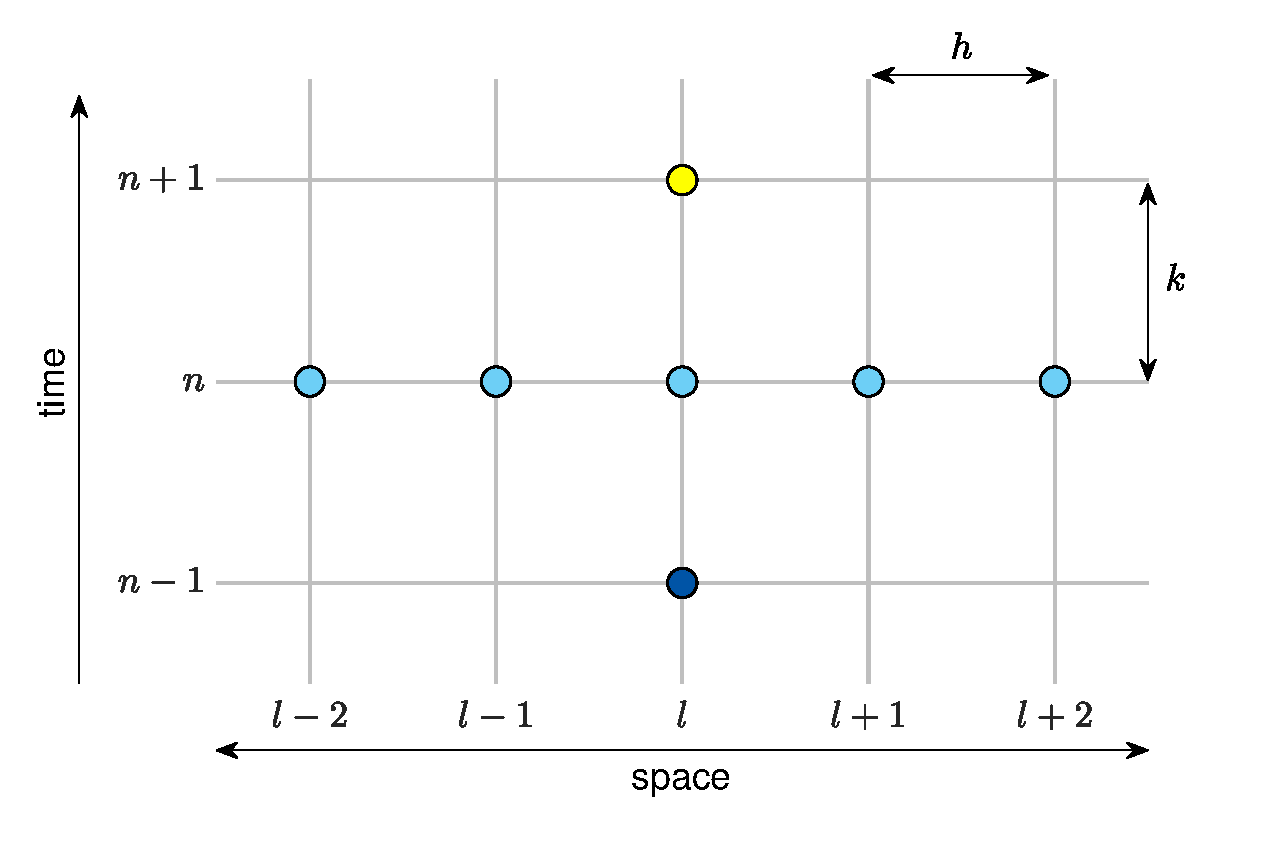
\includegraphics[width=1.0\columnwidth]{stencil1D.eps}
\caption{Stencil for a stiff string finite-difference scheme with grid-spacing $h$ and time-step $k$. The point $l$ at the next time-step (yellow) is calculated using five points at the current time-step (blue) and one at the previous time-step (dark blue). \label{fig:stencil1D}}
\end{figure}


%\textit{Note: In this paper we have used the simple case of a single point for bowing and connections. These can be extended to a bowing area or area of connection. For more information on this, we would like to refer the reader to \cite{Bilbao2009:NumericalSoundSynthesis} for bowing area and \cite{Bilbao2009:ModularPercussion} for area of connection}.
\subsection{Plate}
For the plate, the stencil will consist of 13 grid-points as can be seen in Figure \ref{fig:stencil2D}.

\begin{figure}[h]
\centering
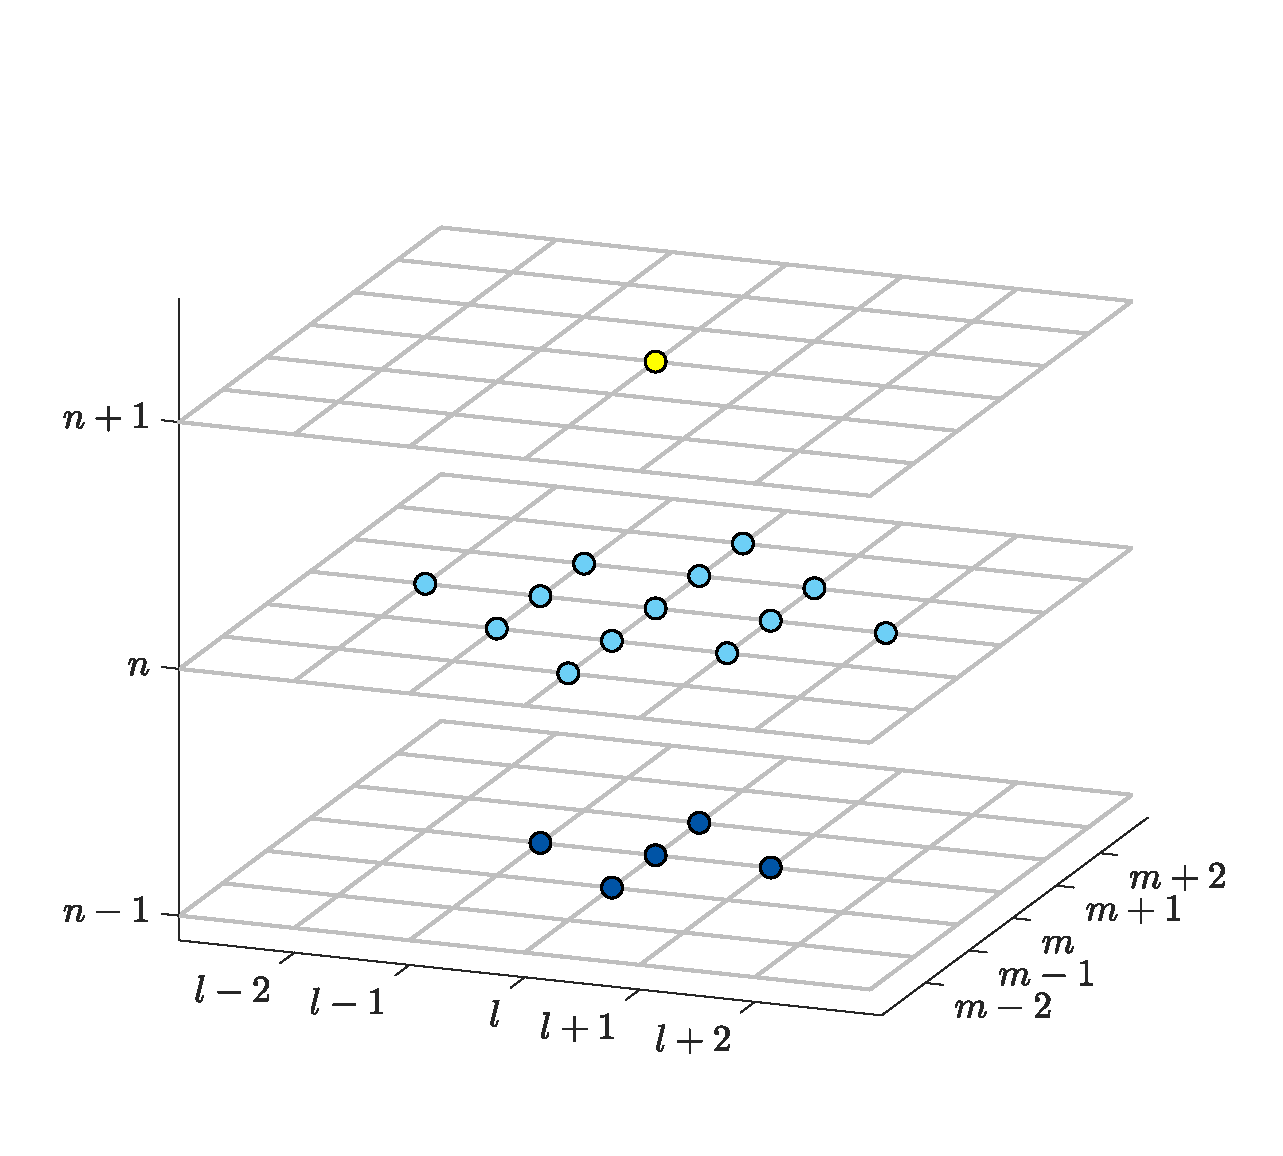
\includegraphics[width=1.0\columnwidth]{stencil2D.eps}
\caption{Stencil for a plate finite-difference scheme. The point $(l,m)$ at the next time-step (yellow) is calculated using 13 points at the current time-step (blue) and five at the previous time-step (dark blue). \label{fig:stencil2D}}
\end{figure}

For stability reasons, the grid-spacing needs to abide the following condition
%section 7.2.3 numerical sound synthesis
\begin{equation}\label{eq:stabilityString}
    h \geq \sqrt{\frac{\gamma^2 k^2 + 4 \sigma_1 k + \sqrt {(\gamma^2 k^2 + 4 \sigma_1 k)^2 + 16 \kappa^2 k^2}}{2}}.
\end{equation}
The closer $h$ is to this limit, the higher the quality of the implementation. The number of points $N$ can then be calculated using 
\begin{equation}
    N = h^{-1}.
\end{equation}

In the case of the plate, calculated the grid spacing using \cite{Bilbao2009:ModularPercussion}
\begin{equation}
h = 2\sqrt{k\bigg(\sigma_1^2 + \sqrt{\kappa^2+ \sigma_1^2}\bigg)}
\end{equation}
after which we calculate $N_x$ and $N_y$ using
\begin{align}
    N_x &= \text{floor}\Bigg(\frac{\sqrt{a}}{h}\Bigg)\\
    N_y &= \text{floor}\Bigg(\frac{1}{h\sqrt{a}}\Bigg)
\end{align}
where $a = N_x / N_y$ is a user-defined length-width ratio.


\subsection{Connections}
The equations in \eqref{eq:connectionsPDE} can be approximated using \cite{Bilbao2009:ModularPercussion}
\begin{subequations}
\begin{align}\label{eq:connectionsFDS}
    F_\alpha &= -\omega_0^2\mu_{t\cdot}\eta - \omega_1^4\eta^2\mu_{t\cdot}\eta - 2\sigma_\times\delta_{t\cdot}\eta,\\
    F_\beta &= -\mathcal{M}_{\alpha/\beta}F_\alpha.
\end{align}
\end{subequations}
The relative displacement $\eta$ between $\alpha$ and $\beta$ can be calculated as
\begin{equation}\label{eq:relativeDisp}
    \eta^n = \sigma_\alpha u_{\alpha, x_{\text{c},\alpha}}^n - \sigma_\beta u_{\beta,x_{\text{c},\beta}}^n,
\end{equation}
where $\sigma_\alpha$ and $\sigma_\beta$ are equal to $h$ in the case of the string and $h^2$ for the plate. In other words, this is the difference between the state of element $\alpha$ at connection point $x_{\text{c},\alpha}$ and the state of element $\beta$ at connection point $x_{\text{c},\beta}$ scaled by their respective (squared) grid-spacings $\sigma_\alpha$ and $\sigma_\beta$. Solving \eqref{eq:connectionsFDS} for $\eta^{n+1}$ yields
\begin{equation} \label{eq:etaNext}
    \eta^{n+1} = p^nF_\alpha+r^n\eta^{n-1},
\end{equation}
where
\begin{subequations}
\begin{align}
    p^n &= \frac{-2}{2\sigma_\times / k + \omega_0^2 + \omega_1^4(\eta^n)^2},\\
    r^n &= \frac{2\sigma_\times / k - \omega_0^2 -\omega_1^4(\eta^n)^2}{2\sigma_\times / k + \omega_0^2 + \omega_1^4(\eta^n)^2}.
\end{align}
\end{subequations}
The next step is to obtain $F_\alpha$ which can be used to easily calculate $F_\beta$. We first obtain values for $u$ by solving \eqref{eq:bowedStringFDS} or \eqref{eq:plateFDS} for $u^{n+1}$ for a string or plate respectively. As, at this point, no connection forces have been added yet, this state is referred to as an intermediate state or $u^\text{I}$. This intermediate state can be used to obtain $\eta^{n+1}$ using \eqref{eq:relativeDisp}:
\begin{equation}
    \eta^{n+1} = \sigma_\alpha u_{\alpha,x_{\text{c},\alpha}}^\text{I} - \sigma_\beta u_{\beta,x_{\text{c},\beta}}^\text{I}
\end{equation}
which can be set equal to \eqref{eq:etaNext}. Solving for connection force $F_\alpha$ yields:
\begin{equation}
    F_\alpha = \frac{r^n\eta^{n-1}-(\sigma_\alpha u_{\alpha, x_{\text{c},\alpha}}^\text{I} - \sigma_\beta u_{\beta,x_{\text{c},\beta}}^\text{I})}{\sigma_\alpha J_\alpha u_{\alpha, x_{\text{c},\alpha}}^\text{I} - \sigma_\beta J_\beta u_{\beta,x_{\text{c},\beta}}^\text{I}-p^n},
\end{equation}
where scaling factor $J$ for element E is defined as
\begin{equation}
    J_\text{E} = \frac{k^2}{1+\sigma_{0,\text{E}}k}.
\end{equation}
% This scaling factor is also used when adding the connection forces to the state $u$ where FDSs \eqref{eq:bowedStringFDS} and \eqref{eq:plateFDS} are extended to:
% \begin{equation}
% \begin{aligned}
%     \delta_{tt}u_l^n &= ... + J_\alpha F_\alpha E_\alpha\ ,\\
%     \delta_{tt}u_l^n &= ... + J_\beta F_\beta E_\beta\ .
% \end{aligned}
% \end{equation}
\section{Implementation}\label{sec:implementation}
%kind of a methods section 
% implementation of FDSs and C++ optimization
In this section, we elaborate more on parameter choices in the previous two sections and present the system architecture of the real-time application. The values for most parameters have been arbitrarily chosen and can - as long as they satisfy the conditions - be changed. We used C++ along with the JUCE framework \cite{JUCE2019} for implementing the physical models and connections in real-time. The main hardware used for testing was a MacBook Pro with a 2.2 GHz Intel Core i7 processor.
The most important thing is to optimise the FDSs as these will be ran at sampling rate. We make sure to only have one multiplication per location of $u$ per time-step ($u_l^n$, $u_{l+1}^{n-1}$ etc) (\textbf{SEE APPENDIX DAFX PAPER}) %<-- needs to be more clear
\subsection{String}
%In order to implement the FDSs presented in Section \ref{sec:FDS} they need to be solved for $u^{n+1}$. Equation \eqref{eq:stringImplementation} found in Appendix A shows a solved finite-difference scheme of Equation \eqref{eq:stiffStringFDS}.


As can be seen from Equation \eqref{eq:descreteRelativeVel} the solution for $v_\text{rel}$ is implicit. It is thus necessary to use an iterative root-finding method such as Newton-Raphson [source].

If simply excited, or plucked in the case of a string, we set the distribution function is to a raised cosine with width $w_\text{e}$ [m]

\begin{equation} \label{eq:distribution}
    E(x) = 
    \begin{cases}
        \hfil \frac{1 - \cos(\frac{2 \pi (x - x_\text{e})}{w_\text{e}})}{2}, & x_\text{e} -  \frac{w_\text{e}}{2} \leq x \leq x_\text{e} + \frac{w_\text{e}}{2} \\
        \hfil 0, &\text{otherwise}
    \end{cases}
\end{equation}
scaled by the excitation function over time with excitation duration $d_\text{e}$ [s]
%numerical sound synthesis Eq. (12.28) or
%On the limits of Eq. (4)
\begin{equation}\label{eq:excitation}
    F(t) = 
    \begin{cases}
        f_\text{e}\frac{1 - \cos(\frac{\pi (t - t_\text{e})}{d_\text{e}})}{2}, & t_\text{e} \leq t \leq t_\text{e}+d_\text{e}\\
        \hfil 0, &\text{otherwise}
    \end{cases}
\end{equation}
with excitation force $f_\text{e}$ [N]. 
A visualisation of this can be found in Figure \ref{fig:exctiation}.


%% Discretised version
% The distribution function is set to a raised cosine with width $w_\text{e}$

% \begin{equation}
%     E(l) = 
%     \begin{cases}
%         \hfil \frac{1 - \cos(\frac{2 \pi (l - l_\text{e})}{w_\text{e}})}{2}, & l_\text{e} -  \frac{w_\text{e}}{2} < l < l_\text{e} + \frac{l_\text{e}}{2} \\
%         \hfil 0, &\text{otherwise}
%     \end{cases}
% \end{equation}
% and scaled by the excitation function over time with excitation duration $d_\text{e}$ [s$^{-1}$]
% \begin{equation}
%     F(n) = 
%     \begin{cases}
%         \frac{1 - \cos(\frac{\pi (n - n_\text{e})}{d_\text{e}})}{2}, & n \geq n_\text{e} \wedge n < n_\text{e}+d_\text{e}\\
%     \end{cases}
% \end{equation}

\begin{figure}[t]
\centering
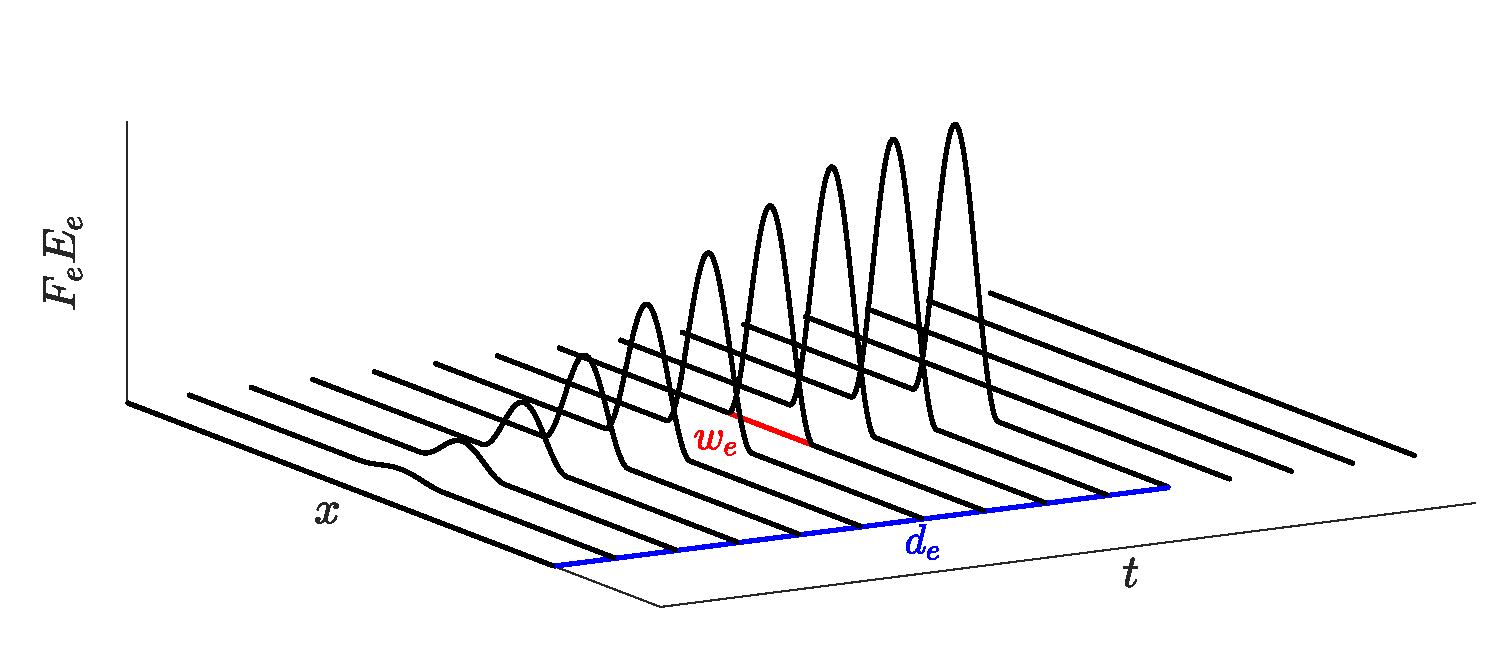
\includegraphics[width=1.0\columnwidth]{excitation.eps}
\caption{A visualisation of the excitation used in our implementation presented in Equation \eqref{eq:excitedString}. The location of excitation $x_\text{e}$ is shown in green, excitation width $w_\text{e}$ in red and excitation duration $d_\text{e}$ in blue (also see Equations \eqref{eq:distribution} and \eqref{eq:excitation}). \label{fig:exctiation}}
\end{figure}

\subsubsection{Frequency}
There are several ways to change the frequency of the string
According to \cite{Bilbao2009:NumericalSoundSynthesis},  the fundamental frequency can be approximately calculated using

\begin{equation}
    f_0 \approx \frac{\gamma}{2}.
\end{equation}

However, as the grid spacing $h$ is dependent on the wave speed $\gamma$ according to the condition found in \eqref{eq:stabilityString}, we must put a lower limit on the number of points $N$ if we plan to dynamically increase $\gamma$.

%maybe it would be better to move the boundary to a different gridpoint and use interpolation for determination of the values around the boundary
Another way to generate different pitches is to add damping to the model at specific points that acts as a fretting finger. The advantage of this is that the condition \eqref{eq:stabilityString} will never be violated. On top of this, a tapping sound will be introduced when fretting the string, making it more realistic than changing the wave speed. If the string is fretted st single location $x_\text{f} \in [0, 1]$ and $l_\text{f} = \text{floor}(x_\text{f}/h)$ we use
\begin{equation}
u_l^n = 
    \begin{cases}
        \hfil 0, & l = l_\text{f} - 1 \vee l = l_\text{f}\\
        \hfil (1-\alpha_\text{f}^\epsilon) u_l^n, & l = l_\text{f} + 1\\
        \hfil u_l^n, & \text{otherwise}
    \end{cases}
\end{equation}
where $\alpha_\text{f} = x_\text{f}/h - l_\text{f}$ describes the fractional location of $x_\text{f}$ between two grid points. Note that the grid point at the finger location and the grid point before, are set to 0 to prevent the states at either side of the finger to influence each other. The disadvantage of using this technique over is that the effect of damping between grid points does not linearly scale to pitch. We thus added $\epsilon = 7$ as a heuristic value to more properly map finger position to pitch.

\subsection{Plate}
An interesting parameter to change is the plate stiffness $\kappa$ as this..

Length-width ratio $a = 2$. 

\subsection{Connections}
As mentioned before, the connections need to be calculated using 

In order to calculate the connection forces $F_\alpha$ and $F_\beta$, the relative displacement of the connection points $E_\alpha$ and $E_\beta$ is needed. We must thus have knowledge of the states of connected elements $\alpha$ and $\beta$. 

\begin{figure}[h]
\centering
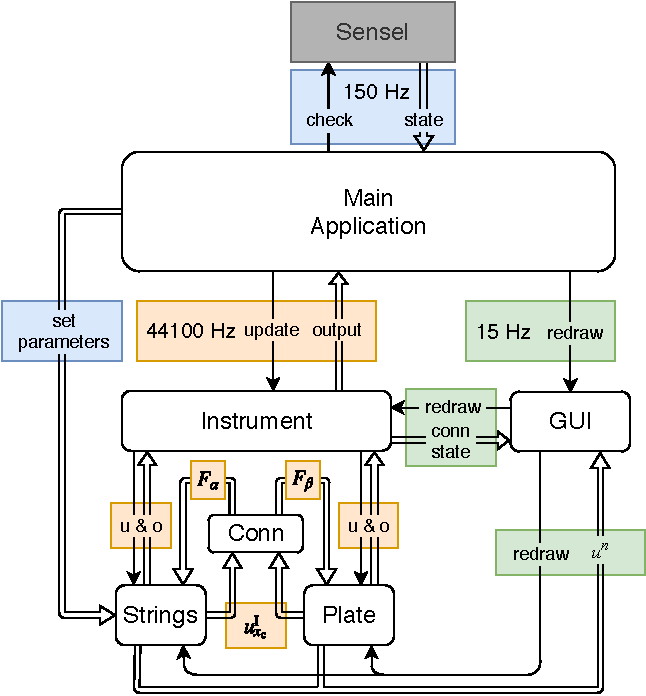
\includegraphics[width=1.0\columnwidth]{JUCE.pdf}
\caption{System architecture flowchart. \label{fig:flowchart}}
\end{figure}

\subsection{System Architecture}
The system architecture can be seen in Figure \ref{fig:flowchart}. The white boxes show the different classes, or components of the application. The hierarchy we adopted can be seen in Figure \ref{fig:hierarchy}.

\begin{figure}[h]
\centering
    \begin{tikzpicture}[level distance=1.3in, sibling distance=.2in,scale=0.75]
    \tikzset{edge from parent/.style= 
        {thick, draw,
            edge from parent fork right},every tree node/.style={draw,minimum width=1in,minimum height=0.25in,text width=1in, align=center},grow'=right}
    \Tree 
    [. {Main App}
        [.{Instrument}
            [. {String} ]
            [. {Plate} ]
            [. {Connection} ]
        ]
    ]
    \end{tikzpicture}
    \caption{System hierarchy. \label{fig:hierarchy}}
\end{figure}
The black arrows in Figure \ref{fig:flowchart} indicate instructions that one class can give to another. The hollow arrows show data flows between classes. All arrows are accompanied by a coloured box indicating on which thread is associated this instruction / dataflow.

The lowest priority thread, the graphics-thread is shown by green boxes and runs at 15 Hz. This draws the states of the instrument strings, connections and the plate on the screen.

Checking and retrieving the Sensel state happens at a rate of 150 Hz and is denoted by blue boxes. The parameters that the user controls by means of the Sensel, such as bowing position, force and velocity, will be updated in the models at the same rate. 

The highest priority thread is the audio-thread and runs at 44100 Hz. The main application gives an 'update' (u) instruction to the instrument which in turn updates the FDSs in its strings and plate. In order to update the states for connected elements, the 

The connection class retrieves the intermediate state $u^\text{I}$ at the connection point $x_\text{c}$ for the two connected elements 

The handling of the data from the sensel is 'converted' into usable parameters and sent to the string models (the plate is not controlled in the applications).
As can be seen in Figure \ref{fig:flowchart}, In order to draw the system, the state needs to be retrieved. This happens on the GUI thread


The most important thing in real-time implementation of FDSs, is to optimise the FDSs themselves as these will be ran at sampling rate. We make sure to only have one multiplication per location of $u$ per time-step ($u_l^n$, $u_{l+1}^{n-1}$ etc) (\textbf{SEE APPENDIX DAFX PAPER}) %<-- needs to be more clear

Furthermore, it is important to take note of is the order of calculation. First the non-extended schemes (Equations \eqref{eq:stiffString} and \eqref{eq:platePDE}) must be calculated before adding the effects of excitations (including bowing), which - in turn - needs to be calculated before adding the effects of connections (see Algorithm \ref{alg:calcOrder}).

\begin{algorithm}[h]\label{alg:calcOrder}
\fbox{\parbox{0.93\linewidth}{
 \While{application runs}{
  calculate intermediate state $u^\text{I}$ for all elements using previous state values
  
  $\quad u^\text{I}_\text{s} = Bu^n + Cu^{n-1}$
  
  \If{element is excited/bowed}{
    calculate excitation term and add to intermediate state of the element
    
    $\quad u^\text{I}_\text{s+e} = u_\text{s}^\text{I} + E$
    }
   \For{all connections}{
   calculate connection forces and add to elements to obtain the state at the next time step
   
   $\quad u^{n+1}_\text{s+e+c} = u_\text{s+e}^\text{I} + C$
   }
  
  update statevectors
  
  $\quad u^{n-1} = u^n$
  
  $\quad u^n = u^{n+1}_\text{s+e+c}$
  
  
  increment time step
  
  $\quad n$++

 }
 }}
 \caption{Pseudocode showing the correct order of calculation. The subscripts for state $u$ shows what it consists of (`s' for previous state, `e' for excitation and `c' for connection).}
\end{algorithm}

\subsection{Sensel Morph}
The Sensel Morph (or further referred to as Sensel) is an expressive touch controller that senses position and force of objects.
% STEFANIA: can you say something more? 
\subsubsection{Mapping strategies}
Something about the different prototype mappings, and the "final" mapping 
Lights to indicate bowing position or string position   
% STEFANIA: add a pictue when we can see one person %interacting with the sensei and we see also the computer's %screen.


\section{Instruments and User Interaction}\label{sec:instruments}
In this section, several configurations of strings, plates and connections that are inspired by real-life instruments will be presented. We subdivide string-elements into three types: bowed, plucked and sympathetic strings. All strings will be connected to one plate which simulates an instrument body. The user can control the plate stiffness and increase it to generate more interaction between the strings. Furthermore, the user can change the output level of each element type. Apart from these parameters, which are controlled by the mouse, the instruments are fully controlled by two Sensels. The instruments we have chosen as our inspiration are the sitar, the hammered dulcimer and the hurdy gurdy. Videos and sound examples can be found through the following link:...

\subsection{User interface}
Strings are shown as coloured paths (also see figures in this section). The state $u$ of the model is visualised using the vertical displacement of the paths. Bowed strings are shown in cyan on the top left. The bow is shown as a yellow rectangle and moves on interaction. The fretting position is shown as a yellow circle. Plucked strings are shown in purple i the top right, underneath which the sympathetic strings are shown in light green. The plate is shown in the bottom using a 18x8 grid of rectangles (clamped gridpoints are not shown). Its state is visualised using a grey-scale.

Furthermore, connections are shown using orange circles/squares for the points of connection and dotted lines between connected elements.

Lastly, all parameters that are controlled by the mouse - output-mix, plate stiffness, etc - are located in a column on the right side of the UI.

\subsection{Bowed Sitar}
The sitar is originally an Indian string instrument that has both fretted strings and sympathetic strings. Instead of plucking the fretted strings, we extended the model to bow these strings. Our implementation consists of 2 bowed strings, 13 sympathetic strings and 5 plucked strings (as it is also possible to strum the sympathetic strings). See Figure \ref{fig:bowedSitar} for a visual of the implementation. One Sensel is vertically subdivided into two sections, one for each bowed string, The first finger registered by the Sensel is mapped to the bow and the second is mapped to a fretting finger on the string controlling pitch. The frets are not implemented as such (the pitch is continuous), but they are visualised for reference. The horizontal position of the first finger is mapped to the bowing position on the string, the vertical velocity  to the bow velocity with a maximum of $v_\text{B} = 0.2$ m/s and the finger force is linked to the excitation function with a maximum of $F_\text{B} = 100$ m/s$^2$. The other Sensel is subdivided into 5 sections mapped to the plucked strings. 

\begin{figure}[h]
\centering
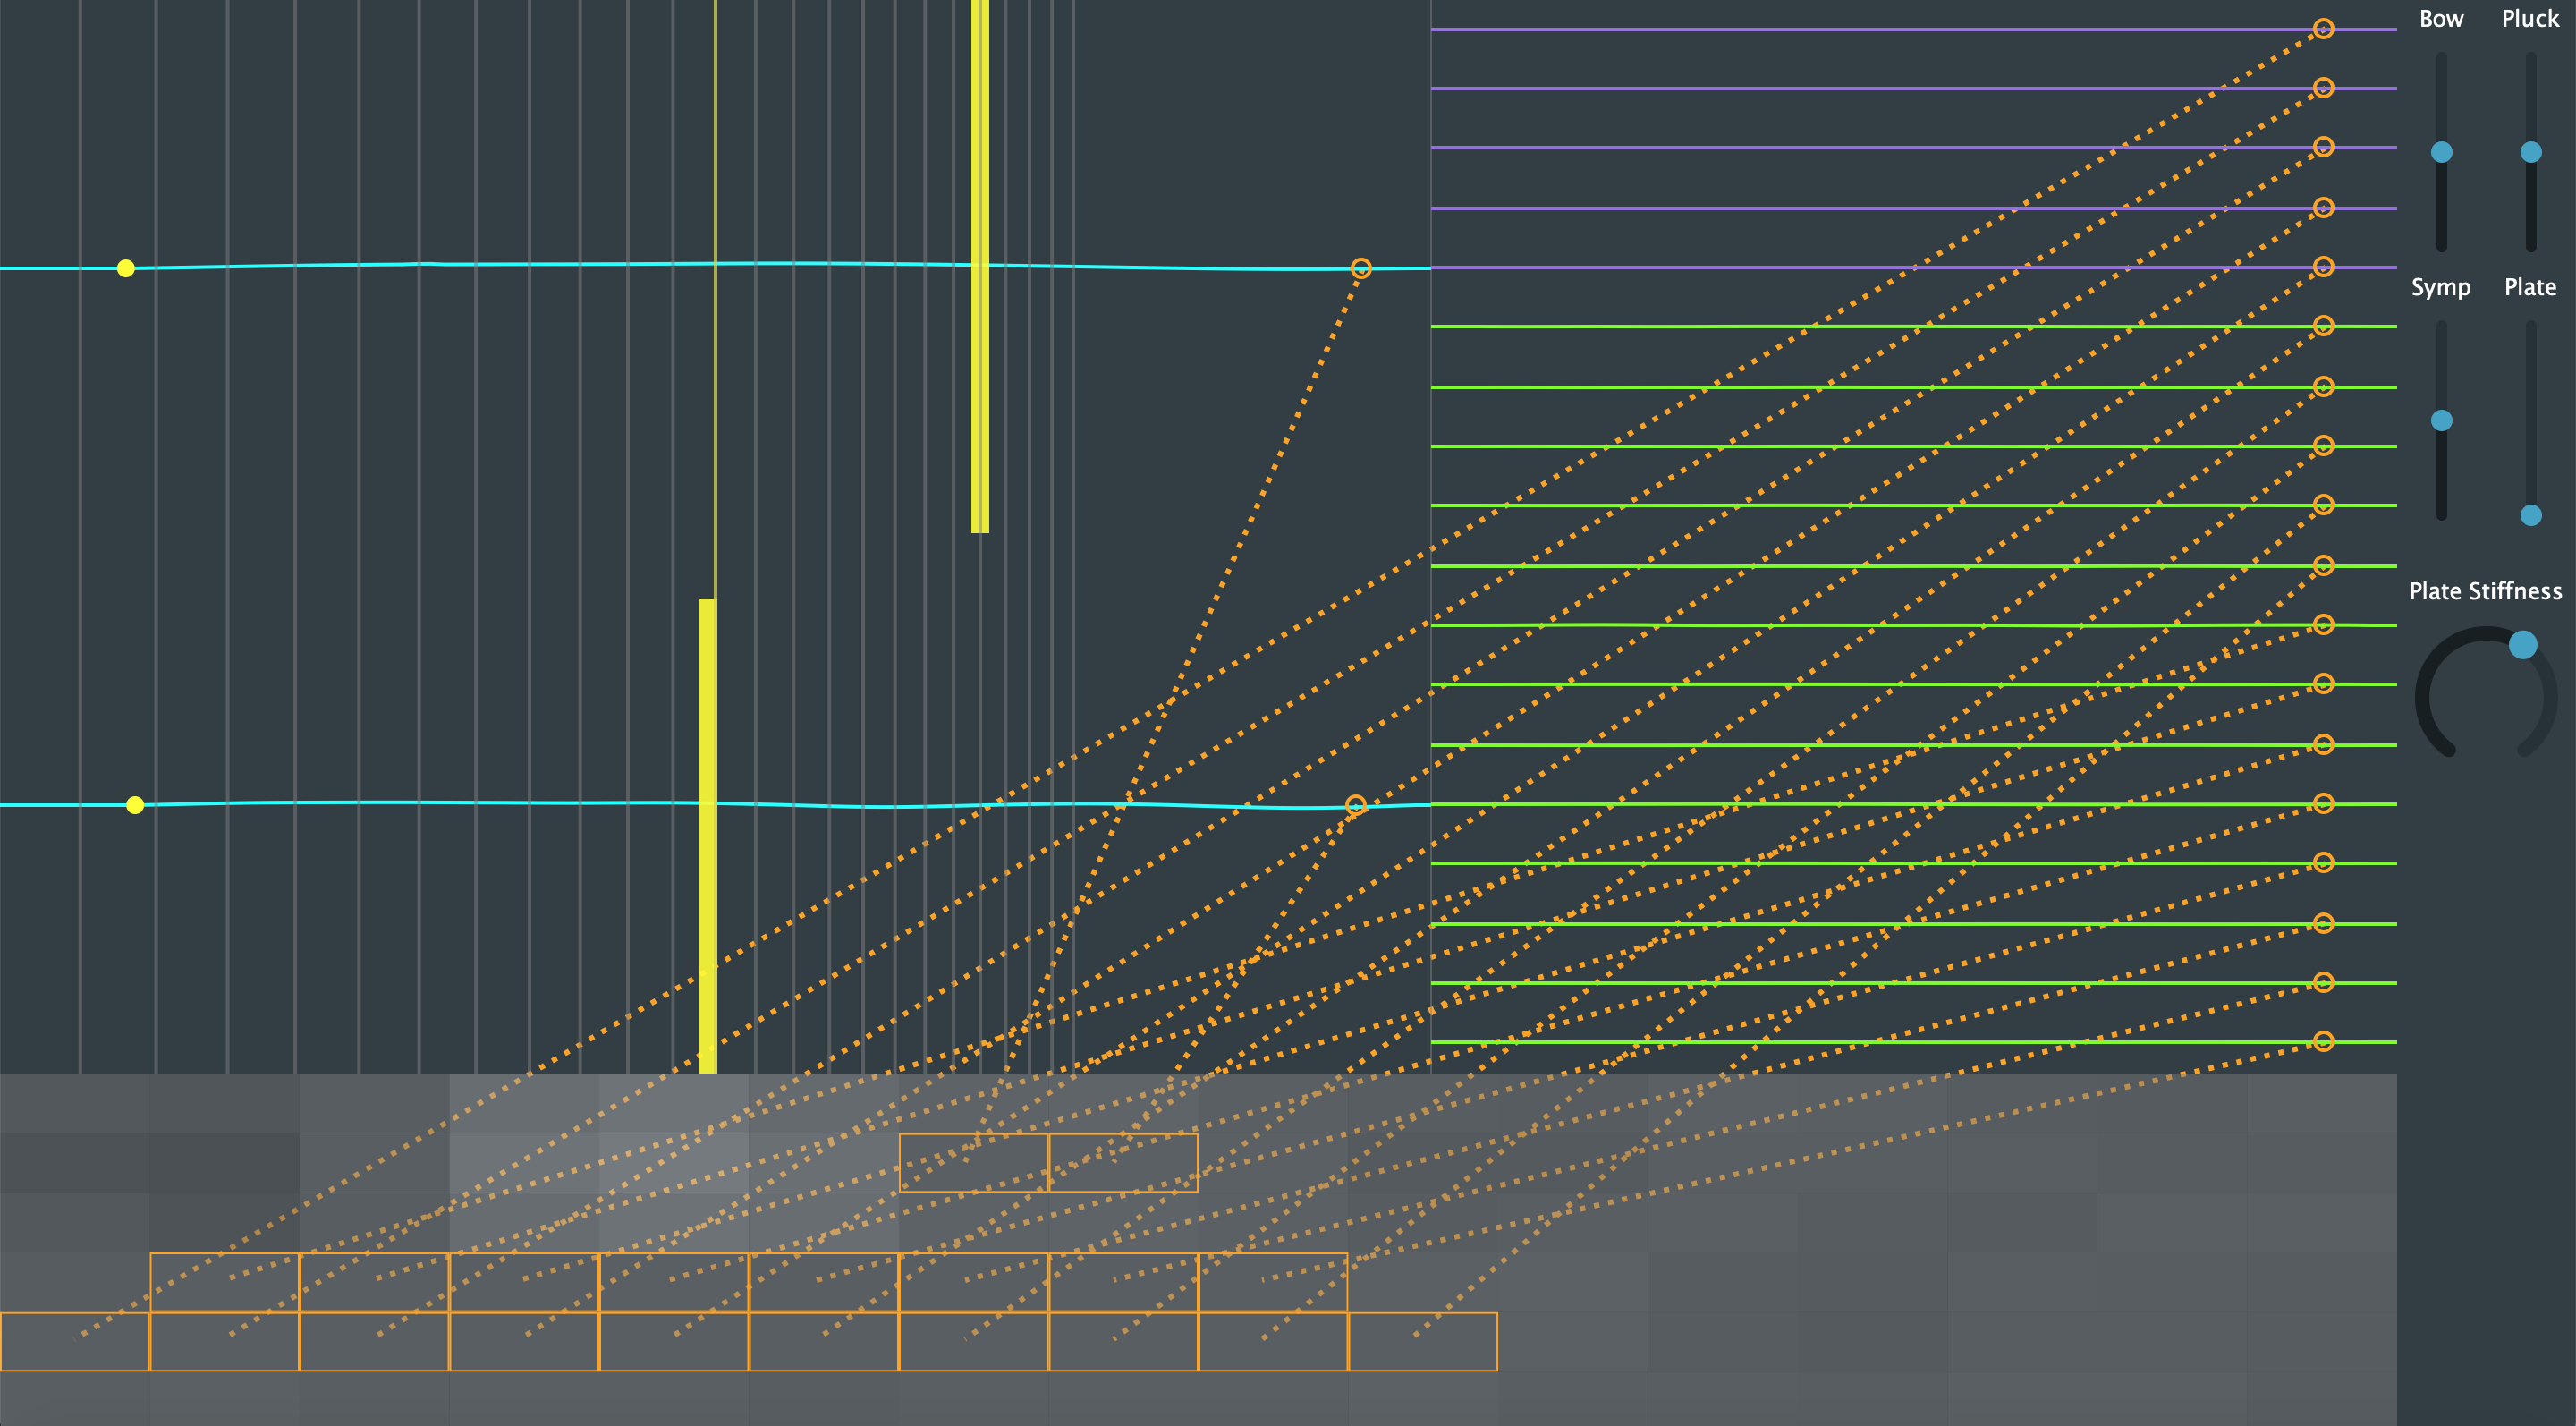
\includegraphics[width=1.0\columnwidth]{BowedSitar.png}
\caption{The bowed sitar application. The descriptions of the different elements and other objects are shown in the image, but will (naturally) not be visible in the application. \label{fig:bowedSitar}}
\end{figure}

\subsection{Hammered Dulcimer}
The hammered dulcimer is an instrument that can be seen as an 'open piano' where the musician has the hammers in their hand. Just like the piano, the strings are grouped in pairs or triplets
that are played simultaneously. 
In our implementation, we have 20 pairs of plucked strings. The excitation (which are plucked strings with a longer excitation length) %need to work on a hammer model 
One of each pair is connected to the plate which slightly detunes it.
% STEFANIA: screenshot of hammered dulcimer model


\subsection{Hurdy Gurdy}
The hurdy gurdy is an instrument that consists of bowed and sympathetic strings. The bowing happens through a rosined wheel attached to a crank and bows these strings as the crank is turned. It is possible to change the pitch of a few bowed strings - the melody strings - using buttons that press tangent pins on the strings at different positions. The other strings, referred to as drone strings, are mostly tuned lower than the melody strings and provide the base notes of the instrument. The musician can place the bowed strings on rests that keep the wheel from interacting with it. 

Our implementation consists of 5 bowed strings subdivided into 2 drone strings tuned to A2, E3 and 3 melody strings tuned to A3, E4 and A4 and 13 sympathetic strings. 

The Sensel is vertically subdivided into 5 rows that control whether the strings are placed on the wheel. The bowing velocity is mapped to the average pressure of the fingers. The pitch (in the model this is the wave-speed $c$) of the melody-strings are changed by a midi controller.
% STEFANIA: screenshot of hurdy gurdy model

\section{Results}
Informal evaluation
CPU usage

\section{Discussion}\label{sec:discussion}

Body should not be plate.
While our instruments have been not formally evaluated yet, noneless we performed some qualitative evaluations with sound and music computing experts.
The goals of the evaluations were to explore the playability of the instrument, sonic quality and intuitiveness of control.
We did an informal test with a lecturer of the Rytmisk Center København 
The interaction with the bow has been found very natural. Bow force and velocity... 

\section{Conclusion and Future Work}\label{sec:conclusion}
Speed up more: AVX vector such as \cite{Webb2015}
Model instrument bodies for more realistic sounds


\begin{acknowledgments}
We would like to thank Stefan Bilbao for his guidance during the course of this project. 
\end{acknowledgments} 

%%%%%%%%%%%%%%%%%%%%%%%%%%%%%%%%%%%%%%%%%%%%%%%%%%%%%%%%%%%%%%%%%%%%%%%%%%%%%
%bibliography here
\bibliography{smc2019bib}
\end{document}
